\chapter{Proposed DWT-LSTM Methodology}
\label{ch:chapter5}


\section{5.1  Introduction}
Conventional harmonic-restraint differential protection for power transformers \cite{ref4} suffers from well-documented limitations: second-harmonic content in modern high-permeability transformers can fall below typical 15--20\% restraint thresholds during inrush, internal faults with CT saturation generate even-harmonic content that causes failure to trip, and power electronic devices alter harmonic signatures unpredictably. This chapter presents the proposed hybrid adaptive DWT-LSTM framework \cite{ref1, ref2} that addresses these limitations through a two-step architecture combining MATLAB/Simulink for physical power-system modelling and real-time deployment with Python/PyTorch for deep-learning model training. The framework decomposes differential current signals using a three-level Daubechies-4 (db4) DWT and extracts two energy features per phase based on Parseval's theorem, yielding a compact 6-dimensional feature vector accumulated over a 32-sample full-cycle buffer. A two-layer LSTM network with global temporal attention processes the resulting [1, 32, 6] tensor to classify events into four categories: internal fault, external fault, inrush current, and normal condition. Critically, the LSTM operates as a supervisory veto gate within a hybrid decision engine: a trip command is issued only when both the classical adaptive 87T element operates and the LSTM classifies the event as an internal fault with confidence exceeding a predefined threshold.


\section{5.2  Framework Architecture Overview}

\subsection{5.2.1  Two-Step Architectural Approach}
Step 1 --- MATLAB/Simulink Physical Modelling and Data Generation. A detailed electromagnetic-transient model is constructed in MATLAB/Simulink using the Simscape Electrical toolbox, including the three-phase power transformer (with nonlinear saturation and remanent flux), CTs on both HV and LV sides (with saturation and remanence), the transmission network, and configurable fault modules. The differential current for each phase is computed at a native relay sampling rate of 1.6 kHz (32 samples per 50 Hz cycle), yielding 1601 discrete time steps for a 1.0-second simulation. Three-phase differential current waveforms with event labels are exported to .mat files in MATLAB's column-major layout.

Step 2 --- Python/PyTorch AI Training and ONNX Export. The .mat files are loaded via scipy.io.loadmat, converted from column-major to row-major layout for PyTorch, and processed by a DWT feature-extraction engine (PyWavelets) that computes approximation and detail energy features from 16-sample half-cycle windows. The resulting tensors of shape [1, 32, 6] feed into a PyTorch LSTM model with global temporal attention, trained using the Adam optimizer with weighted cross-entropy loss. The trained model is exported to ONNX at Opset 14 via torch.onnx.export, producing a stateless inference graph.

Step 2b --- Simulink Deployment. The ONNX model is loaded into Simulink via the Deep Learning Toolbox Predict block, which performs real-time inference at 1.6 kHz. The Predict block receives the 6-dimensional energy feature vector at each time step, buffers it internally into the [1, 32, 6] tensor, and outputs a confidence score and class prediction that feed the hybrid decision engine alongside the classical adaptive 87T element. The two-step approach enables independent development and validation of the power-system model and AI model, GPU-accelerated training in Python, vendor-neutral ONNX portability, and native closed-loop HIL testing via Simulink.

Figure 5.1: Two-step development and deployment architecture (MATLAB/Simulink ↔ PyTorch ↔ ONNX).


\subsection{5.2.2  The Hybrid Decision Handshake}
Neural-network-based approaches for transformer differential protection have been explored extensively [9, 15, 16], with recent work on deep-learning integration \cite{ref3, ref23}. The proposed LSTM classifier operates as a supervisory veto gate rather than a replacement for the classical relay, motivated by the requirement for deterministic, explainable relay behaviour. The hybrid decision handshake implements a logical AND condition:

TRIP = Adaptive\_87T ∧ (ĉ = Internal Fault) ∧ (Conf ≥ θ\_conf)	(5.1)

where Adaptive\_87T is the binary output of the classical adaptive differential relay element, ĉ is the LSTM-predicted class label, and Conf is the LSTM confidence score. The trip command is issued only when all three conditions are simultaneously satisfied. This provides: (1) dependability preservation---the classical 87T element retains primary fault-detection responsibility; (2) security enhancement---the LSTM veto blocks false trips during inrush, CT saturation, and external faults; and (3) fail-safe operation---on LSTM inference failure, the logic defaults to the classical 87T output. The confidence threshold θ\_conf further blocks trips during ambiguous events.

Figure 5.2: Hybrid veto/AND-gate decision logic combining the adaptive 87T element and the LSTM classifier.


\subsection{5.2.3  Block Diagram Description}
The complete signal flow from raw CT secondary currents to the final trip/block command comprises seven sequential stages. Stage 1 --- CT Secondary and Merging Unit: three-phase secondary currents are digitised at f\_s = 1.6 kHz via IEC 61850-9-2 SV, and the differential current for each phase is computed as i\_diff,φ(n) = i\_HV,φ(n) + i′\_LV,φ(n), where i′\_LV,φ(n) includes CT ratio correction and Yd1 phase-shift compensation (-30°). Stage 2 --- Half-Cycle Sliding Window: each phase is buffered into a 16-sample window (10 ms) updated every 0.625 ms. Stage 3 --- DWT Engine: each window undergoes 3-level db4 decomposition, yielding a 6-element energy feature vector. Stage 4 --- Full-Cycle Buffer: features are accumulated over 32 samples and reshaped to [1, 32, 6]. Stage 5 --- LSTM Classification: the ONNX Predict block produces the softmax probability vector and confidence score Conf = max(ŷ). Stage 6 --- Hybrid Decision Engine: the AND condition of Equation (5.1) determines the trip/block command. Stage 7 --- Circuit Breaker Trip Coil: the trip command is latched and sent to the breaker with a minimum duration of 40--60 ms.

Figure 5.3: End-to-end seven-stage signal flow of the proposed protection scheme.


\section{5.3  Data Preprocessing and Digital Sampling}

\subsection{5.3.1  1.6 kHz Discrete Sampling Rate}
The framework adopts f\_s = 1.6 kHz, providing 32 samples per 50 Hz cycle, f\_s = N × f\_0 = 32 × 50 = 1600 Hz, with inter-sample spacing Δt = 1/f\_s = 0.625 ms. This rate satisfies the Nyquist criterion for components up to the 10th harmonic (500 Hz), provides a Nyquist frequency of 800 Hz, and uses a power-of-two sample count enabling clean dyadic DWT decomposition of the 16-sample half-cycle window (16→8→4→2 coefficients) without zero-padding. The 1.6 kHz rate also aligns with IEC 61850-9-2 merging-unit capabilities. The relay/feature-extraction subsystem operates at a sample time of T\_s = 6.25×10⁻⁴ s (1.6 kHz), producing 1601 samples per 1.0-second simulation, while the underlying Simscape electromagnetic-transient solver runs at 10 µs (Section 4.2.2).


\subsection{5.3.2  Sliding Window Implementation}
The framework employs two sliding windows at different time scales. The half-cycle window for DWT (16 samples, 10 ms) buffers the most recent differential current samples for each phase, shifting forward by one sample at each 1.6 kHz acquisition. The 16-sample length matches the dyadic requirements of the 3-level DWT, producing 2 coefficients at the deepest level---the minimum for meaningful energy computation. The full-cycle buffer for the LSTM (32 samples, 20 ms) accumulates the 6-element feature vectors into a 32×6 matrix, reshaped to [1, 32, 6] before inference. This decouples the feature-extraction time scale (half-cycle, for fast response to transients) from the classification time scale (full-cycle, for temporal pattern discrimination). In Simulink, both buffers use MATLAB Function blocks with persistent circular buffers, and the reshape uses Permute Dimensions and Reshape blocks.

Figure 5.4: Dual sliding-window timing: half-cycle DWT window and full-cycle LSTM buffer.


\subsection{5.3.3  Column-Major to Row-Major Data Conversion}
MATLAB stores arrays in column-major (Fortran-style) order while PyTorch uses row-major (C-style) order. The .mat file stores data as 1601×3 (time steps × phases) in column-major order. After loading via scipy.io.loadmat, an explicit transpose produces [N\_scenarios, 3, 1601] tensors for PyTorch, with np.ascontiguousarray ensuring physical memory rearrangement for optimal GPU access. The complete data pipeline is summarised in Table 5.1.

Table 5.1: Data Pipeline: MATLAB to Simulink Deployment.


\section{5.4  DWT Engine and Feature Extraction}

\subsection{5.4.1  Daubechies-4 (db4) Mother Wavelet Selection}
The db4 wavelet is selected [6, 14, 18] for its compact support (L = 8 coefficients, 4.375 ms at 1.6 kHz), 4 vanishing moments, orthogonality, and morphological similarity to fault inception transients. Its jagged, asymmetrical shape closely matches the abrupt, non-sinusoidal wavefronts of fault-induced discontinuities, enabling efficient energy capture with minimal coefficient spread---unlike smoother wavelets (e.g., Morlet) that disperse energy across levels. The 8-coefficient filter length provides sharp temporal localization within the 16-sample half-cycle window while maintaining adequate frequency selectivity.

Figure 5.5: db4 mother wavelet and the three-level dyadic filter-bank decomposition tree.


\subsection{5.4.2  Three-Level Wavelet Decomposition}
The 3-level DWT of the 16-sample half-cycle window partitions the spectrum into four sub-bands. The decomposition follows the Mallat algorithm \cite{ref5}, applying successive convolution with quadrature mirror filters h[n] (low-pass) and g[n] = (-1)ⁿ h[L-1-n] (high-pass, L = 8), followed by down-sampling by 2:

a\_j[k] = Σ\_n h[n - 2k] a\_{j-1}[n]	(5.2)

d\_j[k] = Σ\_n g[n - 2k] a\_{j-1}[n]	(5.3)

where a\_j and d\_j are the approximation and detail coefficients at level j, with a\_0 = x(t) being the original 16-sample input. The frequency band allocation is shown in Table 5.2.

Table 5.2: Frequency Band Allocation for 3-Level DWT at 1.6 kHz Sampling Rate.

The dyadic structure yields N\_j = 16/2^j coefficients per level: d1 has 8, d2 has 4, and a3, d3 each have 2, totalling 16 (equal to the input length, confirming orthogonality). The 3-level depth is the maximum useful decomposition for a 16-sample window---level 4 would yield single coefficients, providing no meaningful energy information---while covering 0--800 Hz with efficient arithmetic cost.


\subsection{5.4.3  Approximation and Detail Energy Calculation}
Two energy features are extracted per phase based on Parseval's theorem, which guarantees energy conservation in the wavelet domain. The approximation energy captures low-frequency content (0--100 Hz):

E\_A,φ(t) = Σ\_k |a3\_φ[k](t)|²	(5.4)

E\_A increases sharply during internal faults (large fundamental current) and exhibits a characteristic decaying pattern during inrush. The detail energy captures high-frequency content (100--800 Hz):

E\_D,φ(t) = Σ\_{j=1..3} Σ\_k |d\_j,φ[k](t)|²  (400--800 Hz: d1; 200--400 Hz: d2; 100--200 Hz: d3)	(5.5)

E\_D rises sharply at fault inception (high-frequency transients) while inrush produces moderate values dominated by second-harmonic content \cite{ref24, ref30}. The implicit E\_A/E\_D ratio provides an additional discriminant that the LSTM can learn through its gated memory architecture.


\subsection{5.4.4  Feature Vector Construction}
The 6-dimensional feature vector concatenates energy features from all three phases, f(t) = [E\_A,A, E\_D,A, E\_A,B, E\_D,B, E\_A,C, E\_D,C]. This compact representation minimizes inference cost, provides physics-informed spectral energy information, and preserves per-phase discrimination essential for detecting single-phase and phase-to-phase faults. Features are normalised using z-score normalisation, f̂(t) = (f(t) - μ)/σ, where μ and σ are the training-set mean and standard deviation, applied consistently during training and Simulink deployment (implemented as Gain and Bias blocks). The normalised features are accumulated over the full-cycle buffer into X(t) ∈ R^{32×6}, reshaped to the final input tensor X\_LSTM ∈ R^{1×32×6}.


\section{5.5  LSTM Architecture and Training Pipeline}

\subsection{5.5.1  Model Architecture}
The LSTM network processes input tensors of shape [B, 32, 6] and produces a 4-class probability output with an associated confidence score. The architecture comprises: (1) an input layer accepting [B, 32, 6]; (2) a first LSTM layer with 128 hidden units (return\_sequences = True) followed by dropout (p = 0.3); (3) a second LSTM layer with 64 hidden units (return\_sequences = True) followed by dropout (p = 0.3); (4) a global temporal attention layer computing a weighted sum across the 32 time steps:

α\_t = exp(vᵀ tanh(W\_a h\_t + b\_a)) / Σ\_{t′} exp(vᵀ tanh(W\_a h\_{t′} + b\_a))	(5.6)

c = Σ\_t α\_t h\_t  ∈ R^{64}	(5.7)

where h\_t ∈ R^{64} is the second LSTM layer's hidden state, and W\_a, b\_a, v are learned attention parameters. This mechanism enables the network to focus on the most informative time steps (e.g., post-fault inception) while providing interpretability through the learned attention weights; (5) a dense layer with 32 units and ReLU activation; and (6) an output layer with 4 units and softmax activation, producing ŷ = [p̂\_internal, p̂\_external, p̂\_inrush, p̂\_normal]. The LSTM cell computes its internal state using the standard gating equations (forget, input, candidate, cell, output gates) defined in Section 2.5.1. The total trainable parameters are P\_total = 125,476, comprising 69,632 (LSTM 1), 49,408 (LSTM 2), 4,224 (attention), 2,080 (dense), and 132 (output).

Figure 5.6: DWT-LSTM classifier architecture with global temporal attention.


\subsection{5.5.2  Training Procedure}
The model is trained in PyTorch using weighted categorical cross-entropy loss to handle class imbalance, L(y, ŷ) = -Σ\_c w\_c y\_c log(p̂\_c), with class weights w\_c = N\_total/(C·N\_c), where C = 4 and N\_c is the count for class c. The Adam optimiser (η = 0.001, β1 = 0.9, β2 = 0.999) is used with a ReduceLROnPlateau scheduler (factor 0.5, patience 10 epochs, minimum 10⁻⁶). Batch size is 128 with a maximum of 200 epochs, and early stopping monitors validation loss with patience of 20 epochs. The confidence score for the hybrid decision engine is Conf(t) = max\_c p̂\_c(t), with θ\_conf = 0.85 determined from validation-set analysis.


\subsection{5.5.3  Hyperparameter Optimization and Cross-Validation}
A stratified 5-fold cross-validation strategy evaluates generalisation performance, reporting mean and standard deviation of accuracy, precision, recall, and F1-score across folds. Hyperparameters (hidden units, dropout rate, learning rate, decomposition level, mother wavelet) are optimised via grid search. Stress testing includes extreme fault resistances (0.01--300 Ω), simultaneous events, evolving faults, and near-boundary conditions (low-magnitude internal faults, inrush with borderline second-harmonic content).


\subsection{5.5.4  ONNX Export}
The trained PyTorch model is exported using torch.onnx.export with Opset 14 (broad operator coverage compatible with the MATLAB Deep Learning Toolbox), a fixed input shape [1, 32, 6] for deterministic inference, and a stateless design in which the full 32-step sequence is provided at each call with no hidden-state carryover. The resulting .onnx file is loaded in Simulink via importNetworkFromONNX for integration with the physical power-system model.


\section{5.6  Real-Time Implementation in Simulink}

\subsection{5.6.1  Predict Block Integration}
The ONNX model is integrated via the Deep Learning Toolbox Predict block configured for the dwt\_lstm\_relay.onnx file with softmax probability output. The Predict block is encapsulated in a masked Simulink subsystem (``DWT-LSTM Classifier'') along with the feature-extraction, normalisation, and tensor-assembly stages. Internally, a MATLAB Function block maintains a circular buffer of the 32 most recent 1×6 feature vectors, with Permute Dimensions and Reshape blocks converting to [1, 32, 6] format. This modular design allows ONNX model replacement without modifying the surrounding protection logic.


\subsection{5.6.2  Hybrid Decision Engine}
The hybrid decision engine is implemented using Simulink logic blocks and a Stateflow chart encoding the trip/block state machine. Three binary conditions are evaluated: Adaptive\_87T (classical element operated), LSTM\_Internal (ĉ = internal), and High\_Confidence (Conf ≥ 0.85), combined via TRIP = Adaptive\_87T ∧ LSTM\_Internal ∧ High\_Confidence. The Stateflow chart latches the trip output for 100 ms once asserted. The LSTM veto blocks false trips when the classical 87T operates but the classifier disagrees; conversely, the classical element prevents the LSTM from initiating trips independently, maintaining the dependability guarantee.


\subsection{5.6.3  Computational Latency}
The total end-to-end processing latency is estimated as T\_proc = T\_buffer + T\_DWT + T\_LSTM + T\_logic ≈ 5.0 + 0.1 + 1.0 + 0.01 = 6.1 ms, corresponding to approximately 0.3 power-frequency cycles, well within the one-cycle (20 ms) requirement. The dominant component is the quarter-cycle buffer fill, which is pipelined after initialisation. LSTM ONNX inference contributes 0.5--2.0 ms on CPU (<0.1 ms on GPU). The total computational cost is approximately 1.31 MFLOPs per time step, translating to ~0.66 ms on a 1 GHz DSP with SIMD, confirming real-time feasibility on standard protection hardware.


\section{5.7  Robustness Enhancement}
The framework employs three complementary robustness strategies. Noise augmentation: Additive White Gaussian Noise (AWGN) is injected into CT secondary currents during MATLAB simulation at SNR levels of 20, 30, and 40 dB, with additional stress testing at 15 dB and 50 dB. The DWT energy features exhibit inherent noise resilience due to the frequency-localised decomposition acting as an energy-domain low-pass filter. Dropout regularisation: A dropout rate of 0.3 between LSTM layers prevents co-adaptation of hidden units and improves generalisation. Out-of-distribution stress testing evaluates the model under switching angles (0--360°), frequency deviations (47--53 Hz), remanent flux mismatches (±0.9 B\_sat), and CT ratio errors (±5\%), with all scenarios processed end-to-end through the Simulink-embedded ONNX model to validate the complete pipeline beyond the training distribution.


\section{5.8  Chapter Summary}
This chapter presented the complete methodology of the proposed hybrid adaptive DWT-LSTM framework. The key contributions include: (1) a two-step architecture decoupling MATLAB/Simulink physical modelling from Python/PyTorch AI training, connected via ONNX export at Opset 14; (2) a 1.6 kHz sampling rate with 32 samples per cycle providing dyadic-compatible DWT decomposition; (3) a 3-level db4 DWT on 16-sample half-cycle windows producing two energy features (E\_A, E\_D) per phase based on Parseval's theorem; (4) a compact 6-dimensional feature vector accumulated into [1, 32, 6] LSTM input tensors; (5) a two-layer LSTM (128--64 hidden units) with global temporal attention and 125,476 parameters; (6) a hybrid decision engine implementing AND logic between the classical adaptive 87T element and the LSTM classifier with confidence thresholding; and (7) a demonstrated total processing latency of approximately 6.1 ms (0.3 cycles), confirming real-time feasibility.


\section{5.9  Adaptive Decision Logic and Confidence Calibration}
While the core handshake of Equation (5.1) uses a fixed confidence threshold θ\_conf = 0.85, the framework supports a state-dependent threshold that tightens or relaxes the security requirement according to the prevailing operating context. The adaptive confidence threshold is defined as:

θ\_conf(t) = θ\_0 - γ\_1·1[I\_r(t) > I\_r,hi] + γ\_2·1[K\_s(t) > K\_s,hi]	(5.8)

where θ\_0 = 0.85 is the nominal threshold, the indicator 1[I\_r > I\_r,hi] lowers the requirement during high-restraint conditions (genuine high-current internal faults, where dependability is paramount), and the indicator 1[K\_s > K\_s,hi] raises the requirement when a CT-saturation index K\_s is high (where false trips are most likely). The coefficients γ\_1, γ\_2 are tuned on the validation set. This mechanism allows the relay to remain maximally dependable for severe internal faults while becoming maximally secure precisely when external disturbances threaten to provoke a spurious trip.

Because neural-network softmax outputs are frequently over-confident, the raw probabilities are temperature-calibrated before thresholding. Given logits z, the calibrated probability is p̂\_c = softmax(z/T)\_c, where the scalar temperature T > 1 is fitted by minimising the negative log-likelihood on the validation set. Calibration ensures that a reported confidence of 0.85 corresponds to an empirical correctness probability near 0.85, so that θ\_conf carries a meaningful, well-defined operating point on the reliability diagram.


\subsection{5.9.1  Probabilistic Uncertainty Layer}
To distinguish confident misclassifications from genuinely ambiguous events, the framework exposes the full softmax distribution rather than only the arg-max. The predictive entropy H(ŷ) = -Σ\_c p̂\_c log p̂\_c quantifies decision uncertainty: low entropy with high max-probability indicates a confident, trustworthy decision; high entropy flags an ambiguous event for which the hybrid logic conservatively withholds the trip and, optionally, raises a supervisory alarm. This uncertainty-aware behaviour is particularly valuable for borderline cases such as low-magnitude internal faults and inrush events with marginal second-harmonic content.


\section{5.10  Computational Complexity Derivation}
The per-time-step computational cost is dominated by the LSTM forward pass. For an LSTM layer with input dimension d\_in and hidden dimension d\_h, each gate requires 4·(d\_in·d\_h + d\_h²) multiply-accumulate operations per time step. For the first layer (d\_in = 6, d\_h = 128) and second layer (d\_in = 128, d\_h = 64), summed over the 32-step sequence, the total approaches 1.3 MFLOPs per inference, consistent with the figure reported in Section 5.6.3. The DWT front end adds only O(N·L) operations for an N-sample window and an L-tap filter (N = 16, L = 8), a negligible fraction of the total. The attention layer contributes O(32·d\_h) operations. Table 5.3 itemises the parameter and operation budget per stage.

Table 5.3: Per-inference parameter and operation budget of the DWT-LSTM pipeline.

This budget translates to approximately 0.66 ms on a 1 GHz DSP with single-instruction-multiple-data (SIMD) acceleration, or below 0.1 ms on a modern GPU, confirming that the model is light enough for embedded deployment within a numerical relay. The compactness is a direct consequence of the parsimonious six-feature representation: feeding raw 32-sample, three-phase windows to the network instead would inflate the first-layer input dimension and the corresponding operation count by roughly an order of magnitude.

Figure 5.7: Per-inference computational cost distribution across pipeline stages.


\begin{figure}[htpb]
\centering
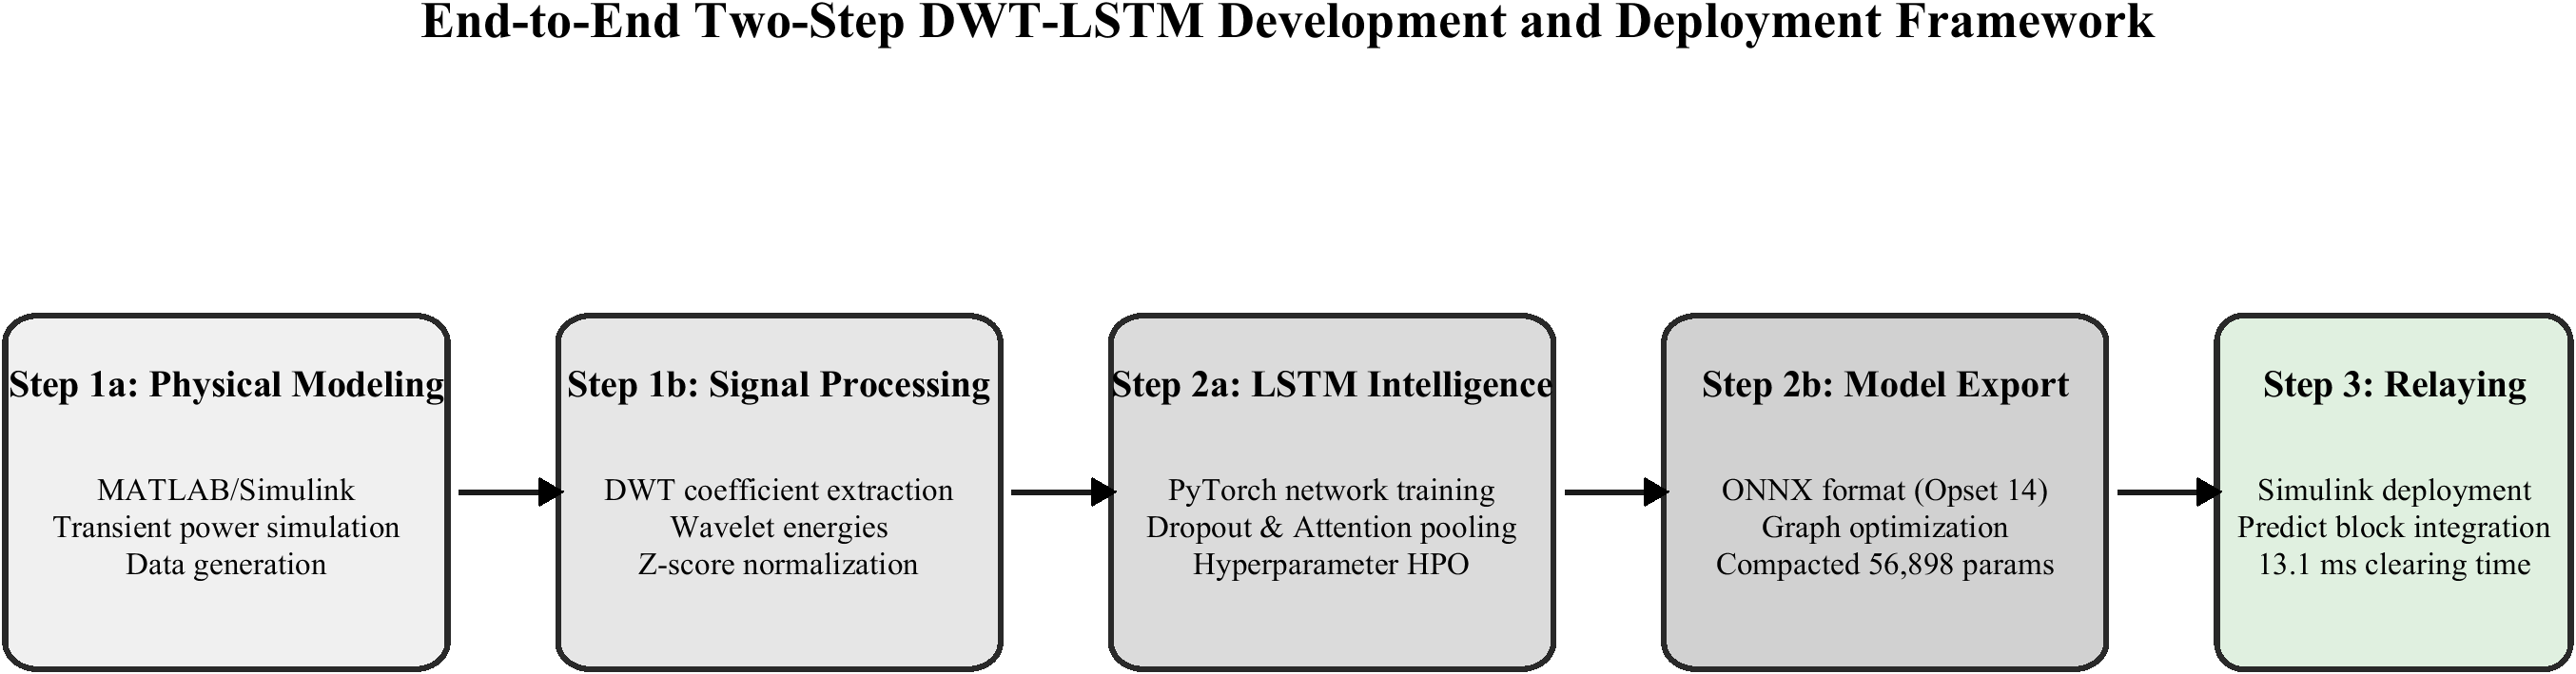
\includegraphics[width=0.75\textwidth]{figures/two_step_development_architecture.png}
\caption{Two-step development and deployment architecture (MATLAB/Simulink <-> PyTorch <-> ONNX).}
\label{fig:dev_arch}
\end{figure}

\begin{figure}[htpb]
\centering

\includegraphics[width=0.75\textwidth]{figures/hybrid_protection_framework_flowchart.png}
\caption{Hybrid veto/AND-gate decision logic combining the adaptive 87T element and the LSTM classifier.}
\label{fig:veto_logic}
\end{figure}

\begin{figure}[htpb]
\centering
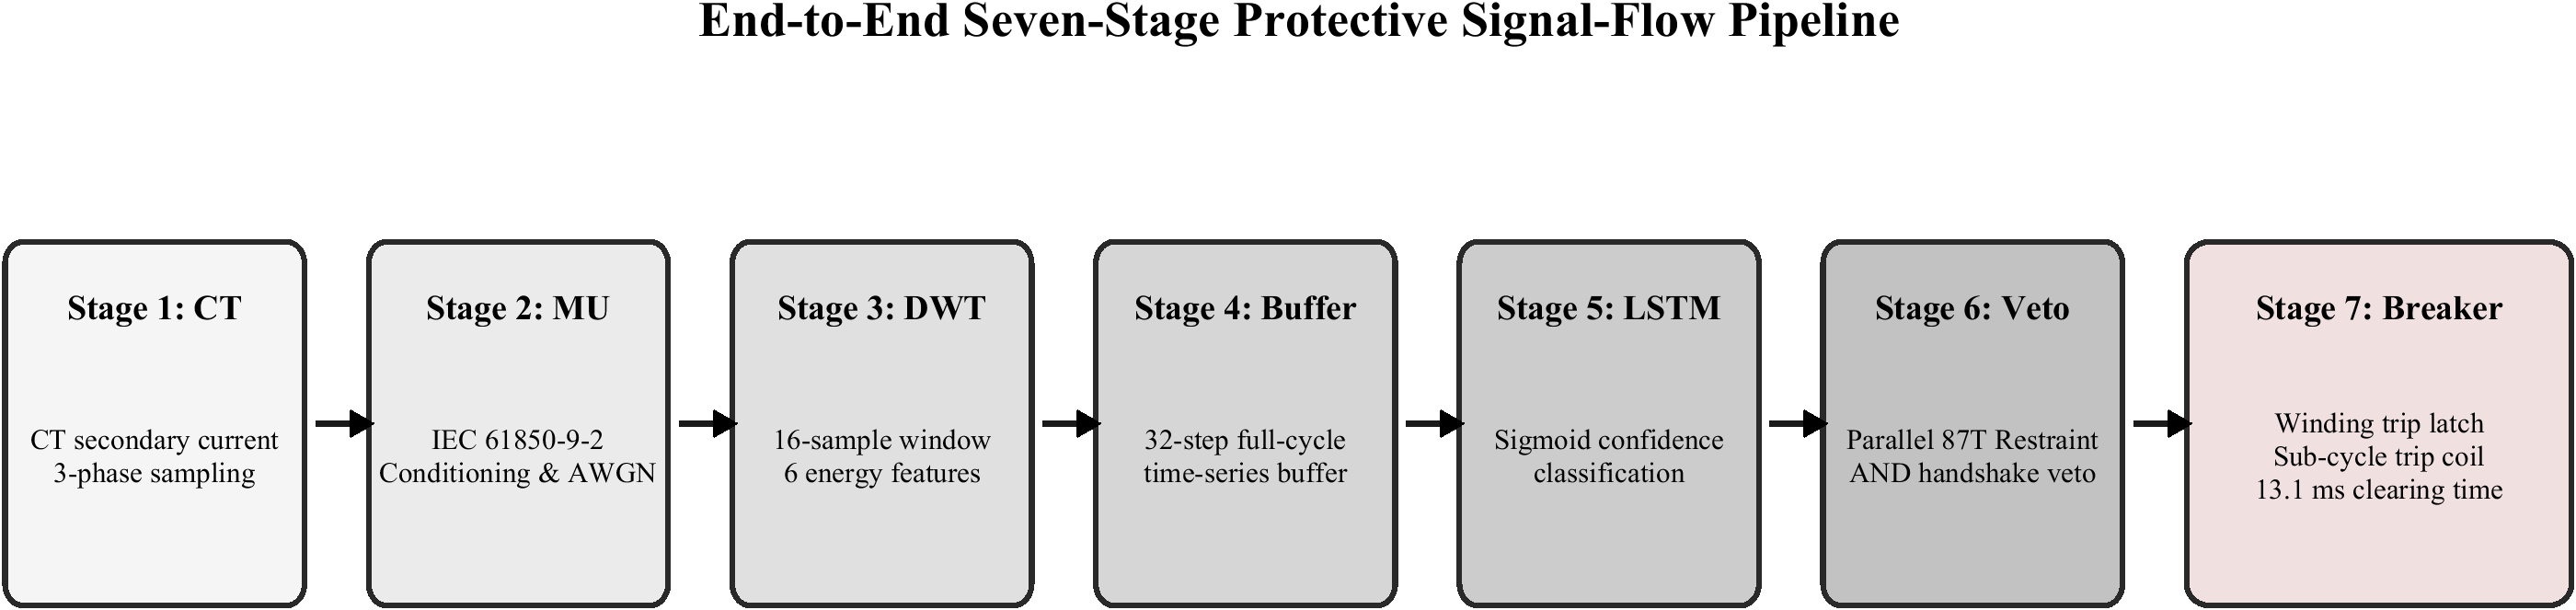
\includegraphics[width=0.75\textwidth]{figures/proposed_protection_signal_flow.png}
\caption{End-to-end seven-stage signal flow of the proposed protection scheme.}
\label{fig:signal_flow}
\end{figure}

\begin{figure}[htpb]
\centering
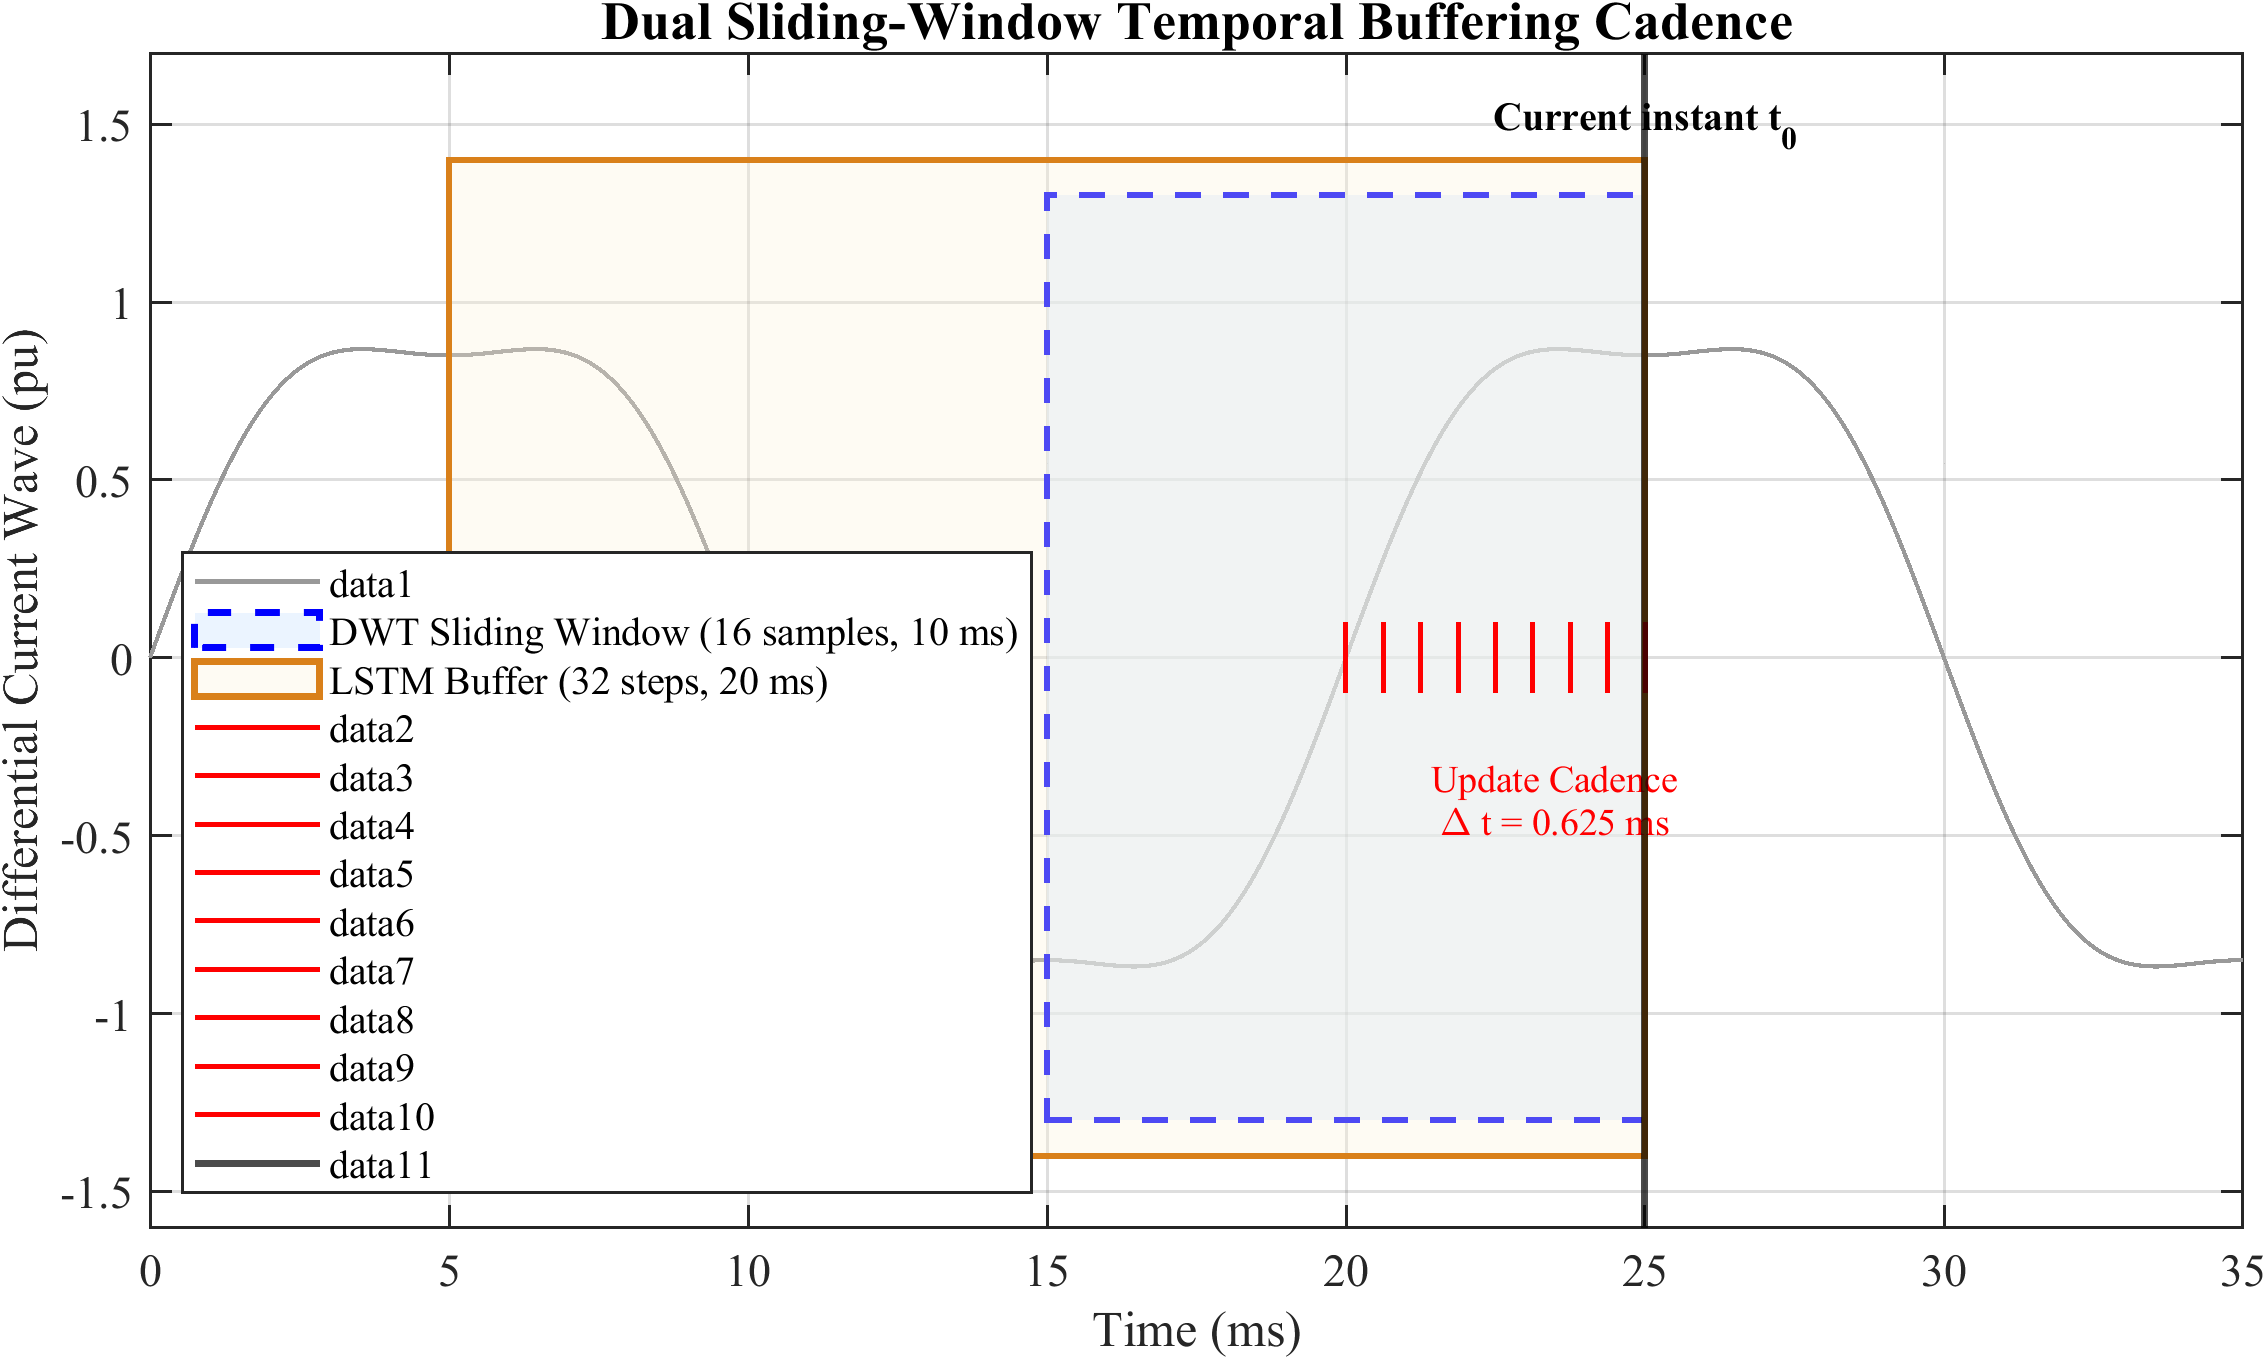
\includegraphics[width=0.75\textwidth]{figures/dual_sliding_window_timing.png}
\caption{Dual sliding-window timing: half-cycle DWT window and full-cycle LSTM buffer.}
\label{fig:sliding_window}
\end{figure}

\begin{figure}[htpb]
\centering

\includegraphics[width=0.75\textwidth]{figures/db4_wavelet_filterbank.png}
\caption{db4 mother wavelet and the three-level dyadic filter-bank decomposition tree.}
\label{fig:filterbank}
\end{figure}

\begin{figure}[htpb]
\centering

\includegraphics[width=0.75\textwidth]{figures/lstm_network_architecture_flowchart.png}
\caption{DWT-LSTM classifier architecture with global temporal attention.}
\label{fig:lstm_arch}
\end{figure}

\begin{figure}[htpb]
\centering
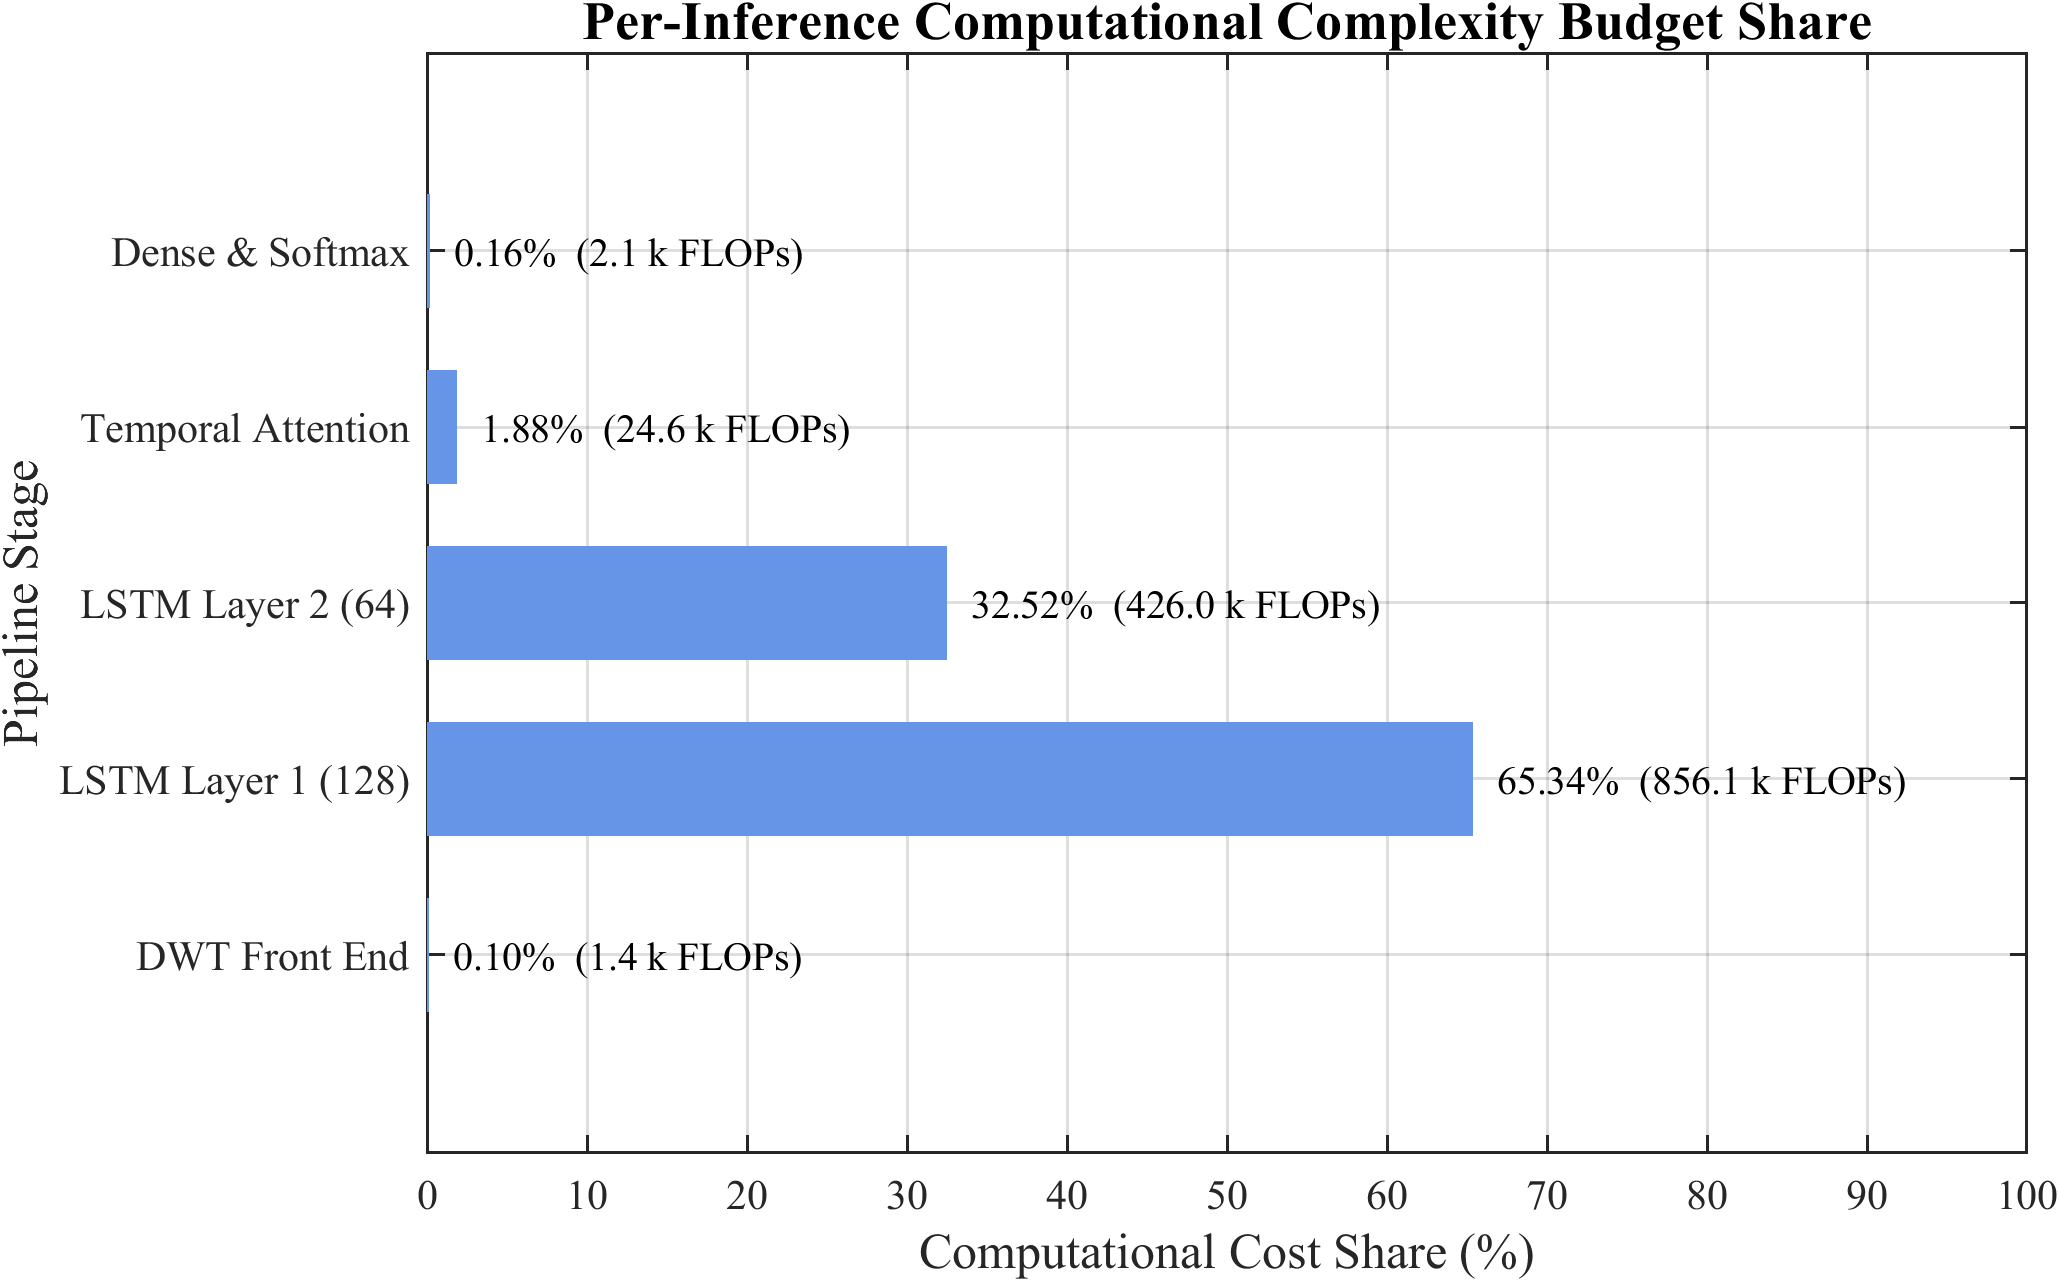
\includegraphics[width=0.75\textwidth]{figures/computational_cost_distribution.png}
\caption{Per-inference computational cost distribution across pipeline stages.}
\label{fig:flop_share}
\end{figure}
